\section{Related work}

Read cascade neural net for inspiration to this introduction

Over the last couple of years an increasing interest in reducing the inference time of intelligent applications to be able to run on less powerful mobile and \gls{iot} device in real-time applications. The survey \citetitle{zhou_edge_2019} by \citet{zhou_edge_2019} review the current state within the research field of \gls{ei}. The survey includes training and inference of \gls{dnn} on the edge and categorizes similar approaches to improve training \gls{ei} application and services and proposals to shorten the inference time in such setups. This thesis is mainly concerned with reducing inference time.

\subsection{Model Architectures}

To improve inference latency on a model-basis, efforts have been made in designing \gls{dnn}s, that efficiently runs on mobile device. Commonly for \gls{mobilenet} \cite{howard_mobilenets:_2017}, \gls{mobilenetv2} \cite{sandler_mobilenetv2:_2018}, \gls{shufflenet} \cite{zhang_shufflenet:_2017} and \gls{shufflenetv2} \cite{ma_shufflenet_2018} are all aiming to efficiently reducing the number of parameters, without compromising model accuracy by designing novel \gls{dnn} architectures.

Use MobileNet's inverted Linear bottlenek as example and use source that describes the parameter efficiency og this model. 

\citeauthor{sandler_mobilenetv2:_2018} designed \textsl{MobileNetV2} is a neural network architecture specifically for mobile devices. The main novelty is \textit{"inverted residual with linear bottlenecks"} a neural network layer module. ELABORATE

Furthermore it uses another type of convolutional layer \textit{depth-wise separable convolutions}, both of which seeking to decrease the number of parameters. ELABORATE

Other efforts have been made to reduce the number of parameters, thus the inference time in state-of-the-art model compression. 

\subsection{Model Compression}

Weight pruning is the removal of redundant weights, which have shown significant speed-ups using with a small loss in accuracy \cite{zhou_edge_2019}. The impact of compression is application dependent and can be applied to any pre-trained \gls{dnn} \cite{cheng_survey_2017}.

Another compression technique is quantization. A more compact representation of a floating point is used to reduce the amount of bits needed for each weight of the model \cite{cheng_survey_2017}. The extreme case is binarization, where weights and activations are learned as a single bit representation. In BinaryConnect \cite{courbariaux_binaryconnect:_2015} and \gls{bnn} \cite{courbariaux_binarized_2016} most arithmetic operations are replaced with bit-wise operations, thus greatly improving the power-efficiency and inference latency, however using binary weights in extremely deep network have shown significant degradation in accuracy \cite{cheng_survey_2017}.

In \cite{hinton_distilling_2015} \gls{kd} has been proposed. \gls{kd} is a framework to train \gls{dnn} in a student-teacher paradigm. The student network are penalized using the output of an ensemble of teacher networks. \gls{kd} can be viewed as a compression of an ensemble of teacher network into a student network \cite{cheng_survey_2017}. 
In \cite{romero_fitnets:_2014} \gls{fitnet} have been proposed as a method to train thinner and shallower student networks using a deeper teacher network. FitNet learns the student network to mimick the teacher network, however this approach require the softmax loss function, which limits is usage \cite{cheng_survey_2017}.  

Other approaches specifically related to edge computing aiming to reduce inference latency, is model partitioning between end device and edge server. 

\subsection{Model Partitioning}

Model partitioning is an approach to reduce inference latency on an architectural level. Instead of solely executing a \gls{dnn} in the cloud, edge or on device, the computing resources collaborates to boost inference time. 

Splitting a model is an inherent nature of sequential \gls{dnn}s, that at any layer can be stopped. The intermediate output are transferred over the network and continued at the next layer on an edge server, as shown in figure \ref{fig:offlaoding}.

\begin{figure}
	\centering
	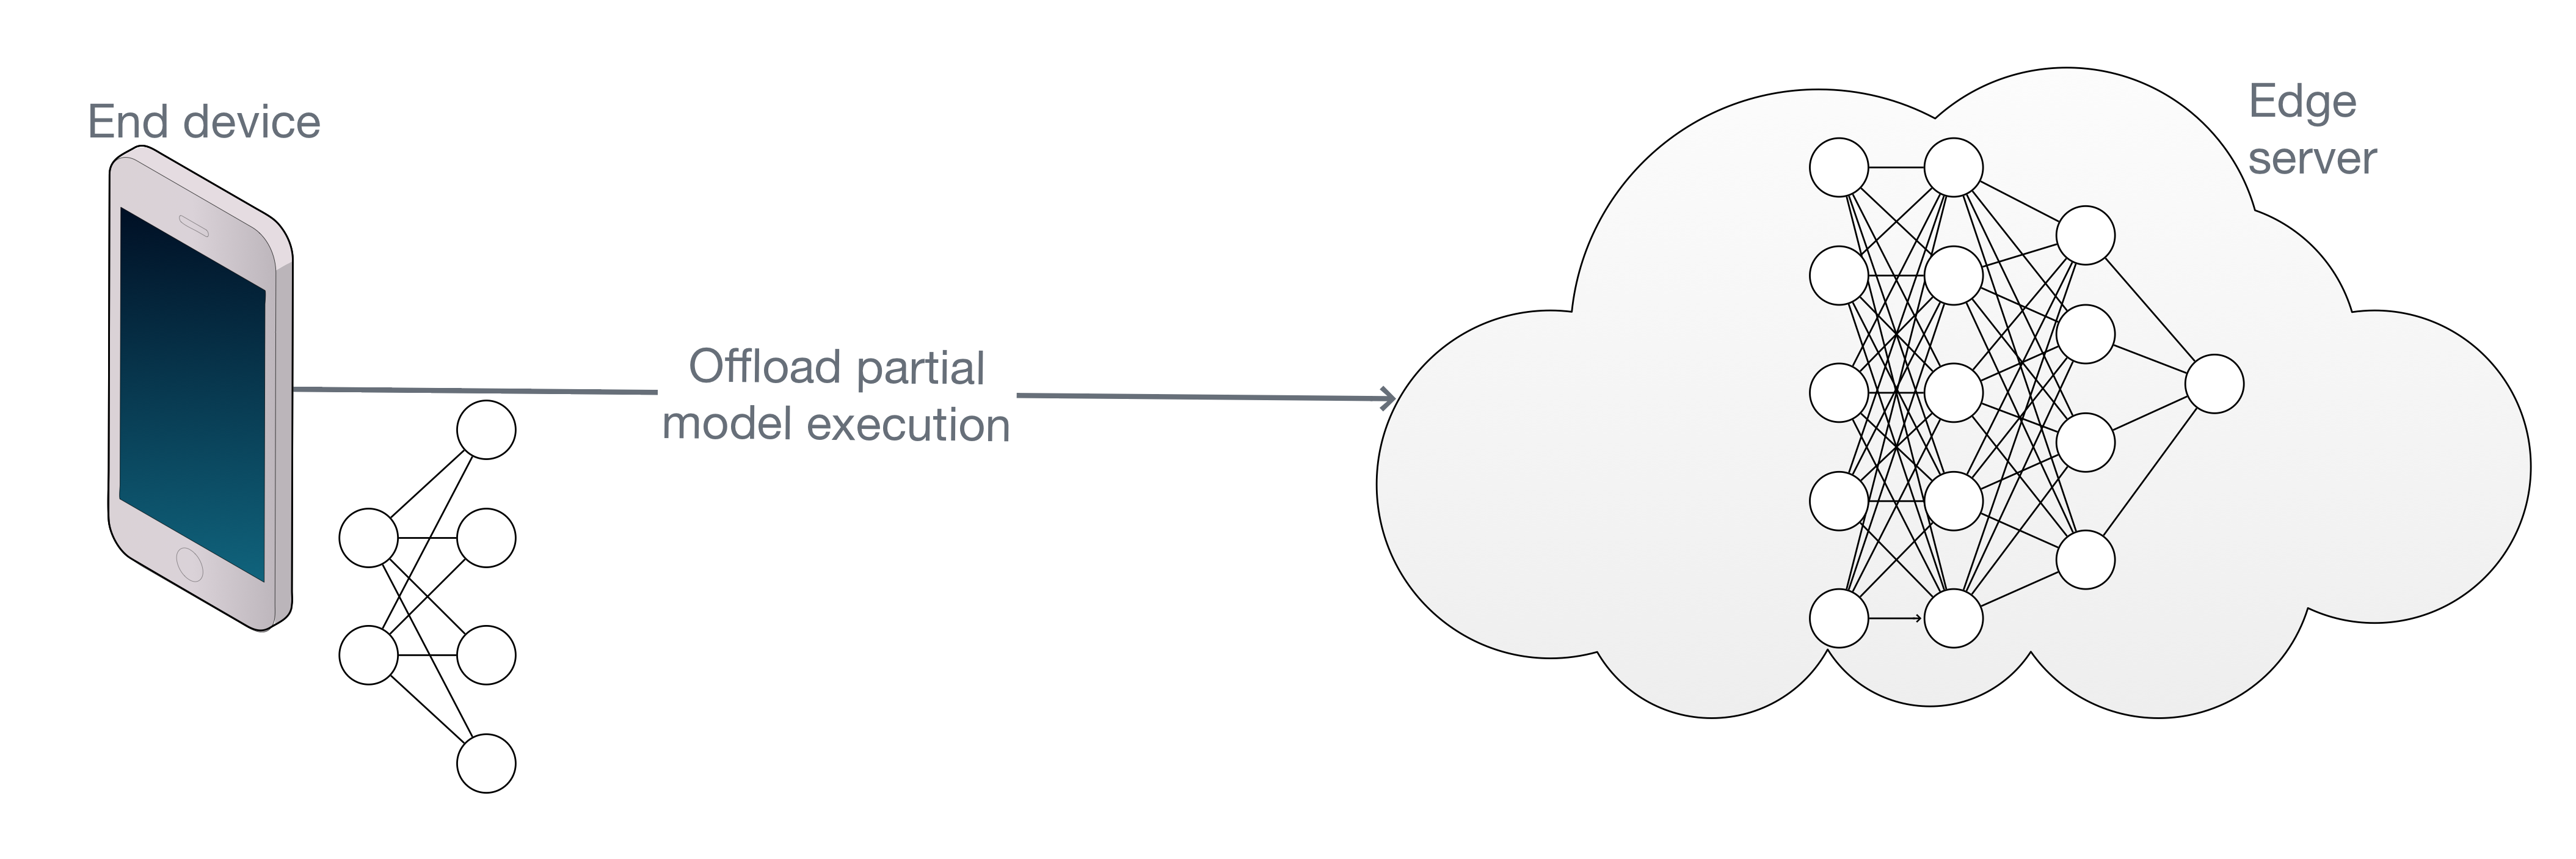
\includegraphics[width=\linewidth]{figures/models/partitioning}
	\caption[Model partitioning]{Edge-Device model partitioning run part of the model on-device and offload the rest to edge processing. Network partitioning utilize the assumption, that at some later point in the \gls{dnn} a smaller representation of the data is found, illustrated by the gradually decreasing model layers, to reduce the communication bottleneck. }
	\label{fig:offlaoding}
\end{figure}

Neurosurgeon \cite{kang_neurosurgeon:_2017} is a lightweight partitioning scheduler, that uses knowledge of the individual layers of the \gls{dnn} to effectively reduce inference latency. Communication latency is the bottleneck in an offloading application, hence a smaller representation of the input data is needed, however the layers producing a smaller output than the original input typically lies deep within the network. Neurosurgeon construct regression models for layer execution time and  output data size of the layers of a \gls{dnn}, to decide the best partition of the \gls{dnn} based on networking condition. The work is based on \gls{mcc} and shows, that the conventional cloud-only approach is insufficient due to different networking technologies and mobile device is becoming \gls{gpu} enabled. 
% Evidently moving computation to the edge reduces the communication latency. 

Another effort to reduce communication overhead of network splitting is adding feature compression of intermediate features before offloading to cloud \cite{choi_deep_2018}. The paper shows, that lossless compression have no impact on accuracy, however bit saving is rather limited. Lossy compression, on the other hand, results in 70\% bit savings, however also affects accuracy and require compression-aware training to compensate. The follow up paper \cite{choi_near-lossless_2018} propose compression techniques for deep features and achieve significant better bit saving, than conventional image compression algorithms.

\begin{figure}
	\centering
	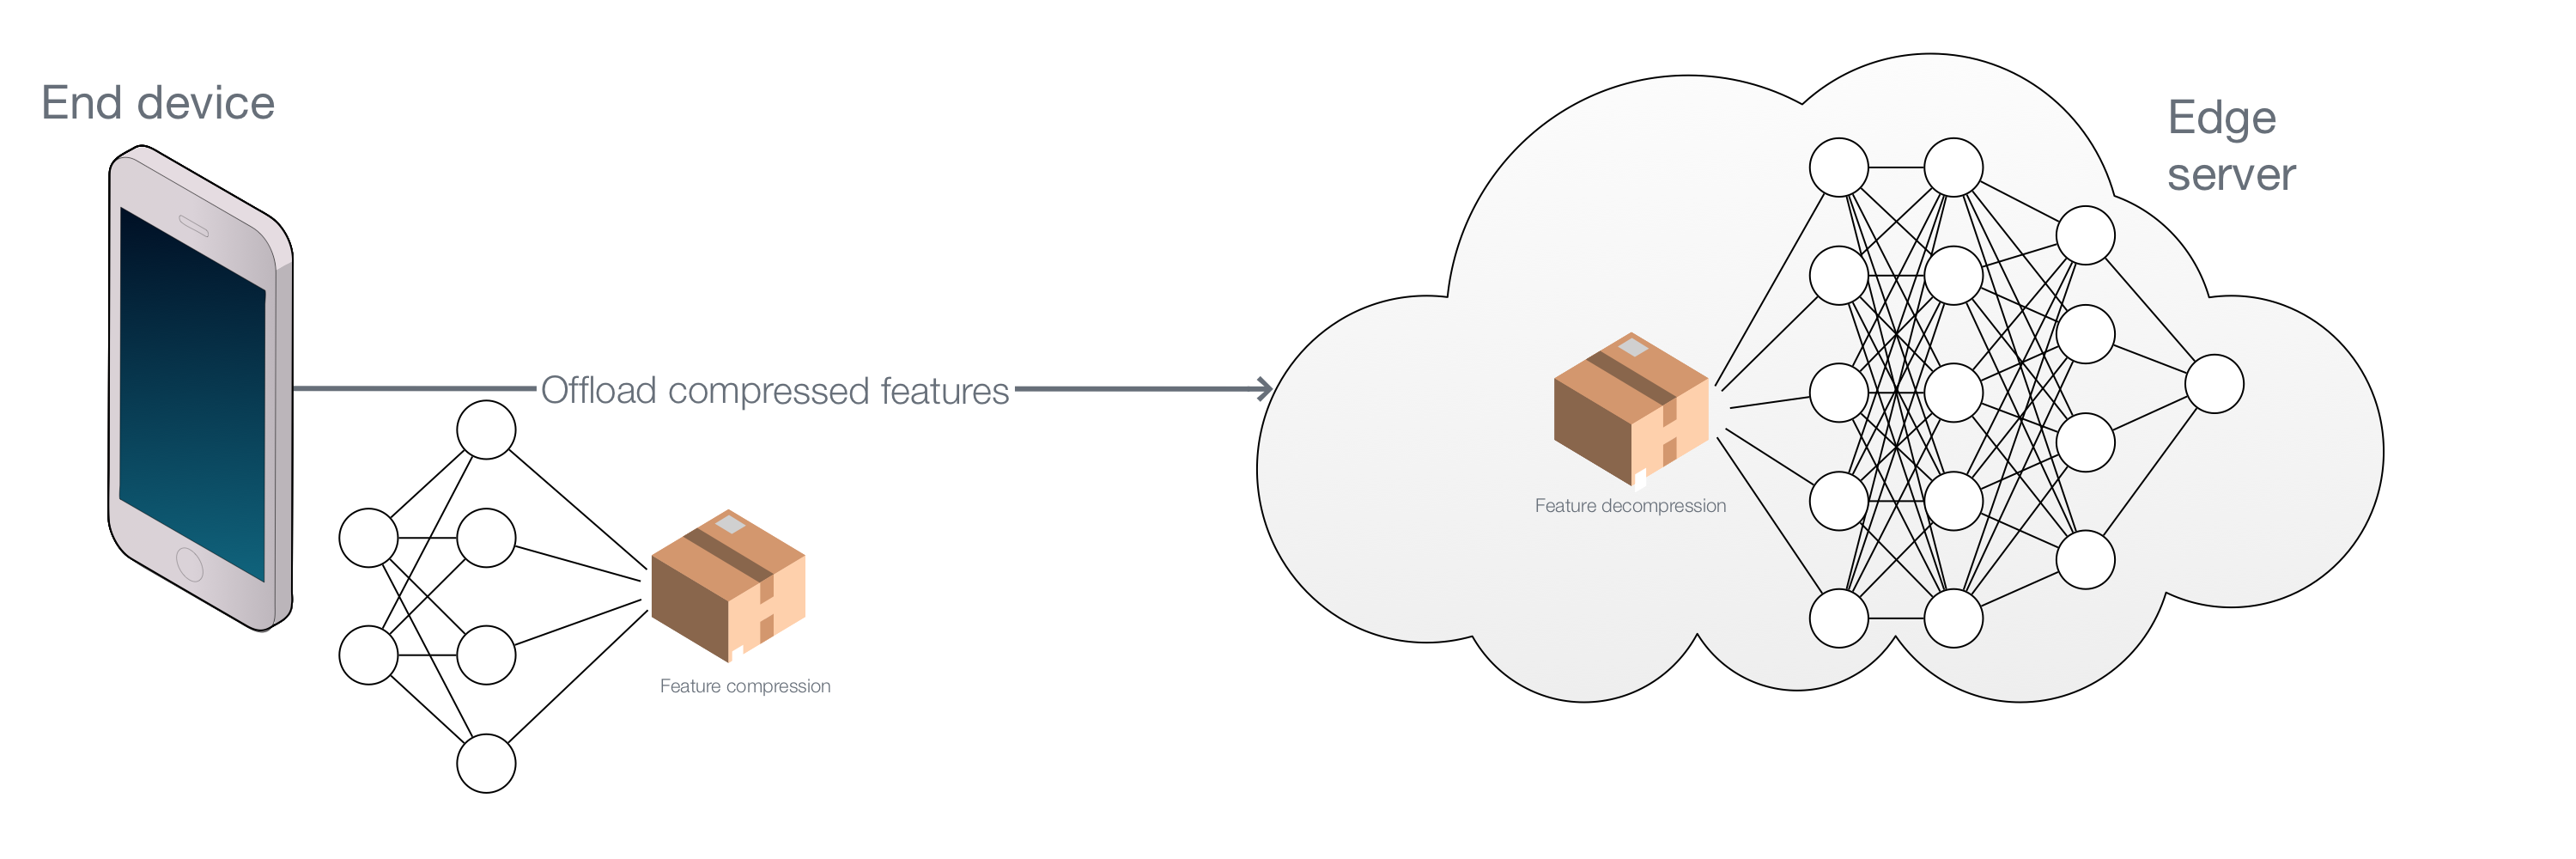
\includegraphics[width=\linewidth]{figures/models/compressed}
	\caption[Feature compression]{Feature compression}
\end{figure}

\gls{bottlenet} \cite{eshratifar_bottlenet:_2019} is a novel neural network module. Client-side it consists of a reduction unit and a compressor unit and server-side of a decompressor unit and restoration unit. The reduction unit creates a smaller representation of intermediate result by applying spatial- and channel-wise convolution. The compressor uses lossy \gls{jpeg} compression, that are decompressed server-side. The restoration unit apply deconvolution to restore the intermediate feature back to the required dimensionality for the next layer in the network.

\begin{figure}
	\centering
	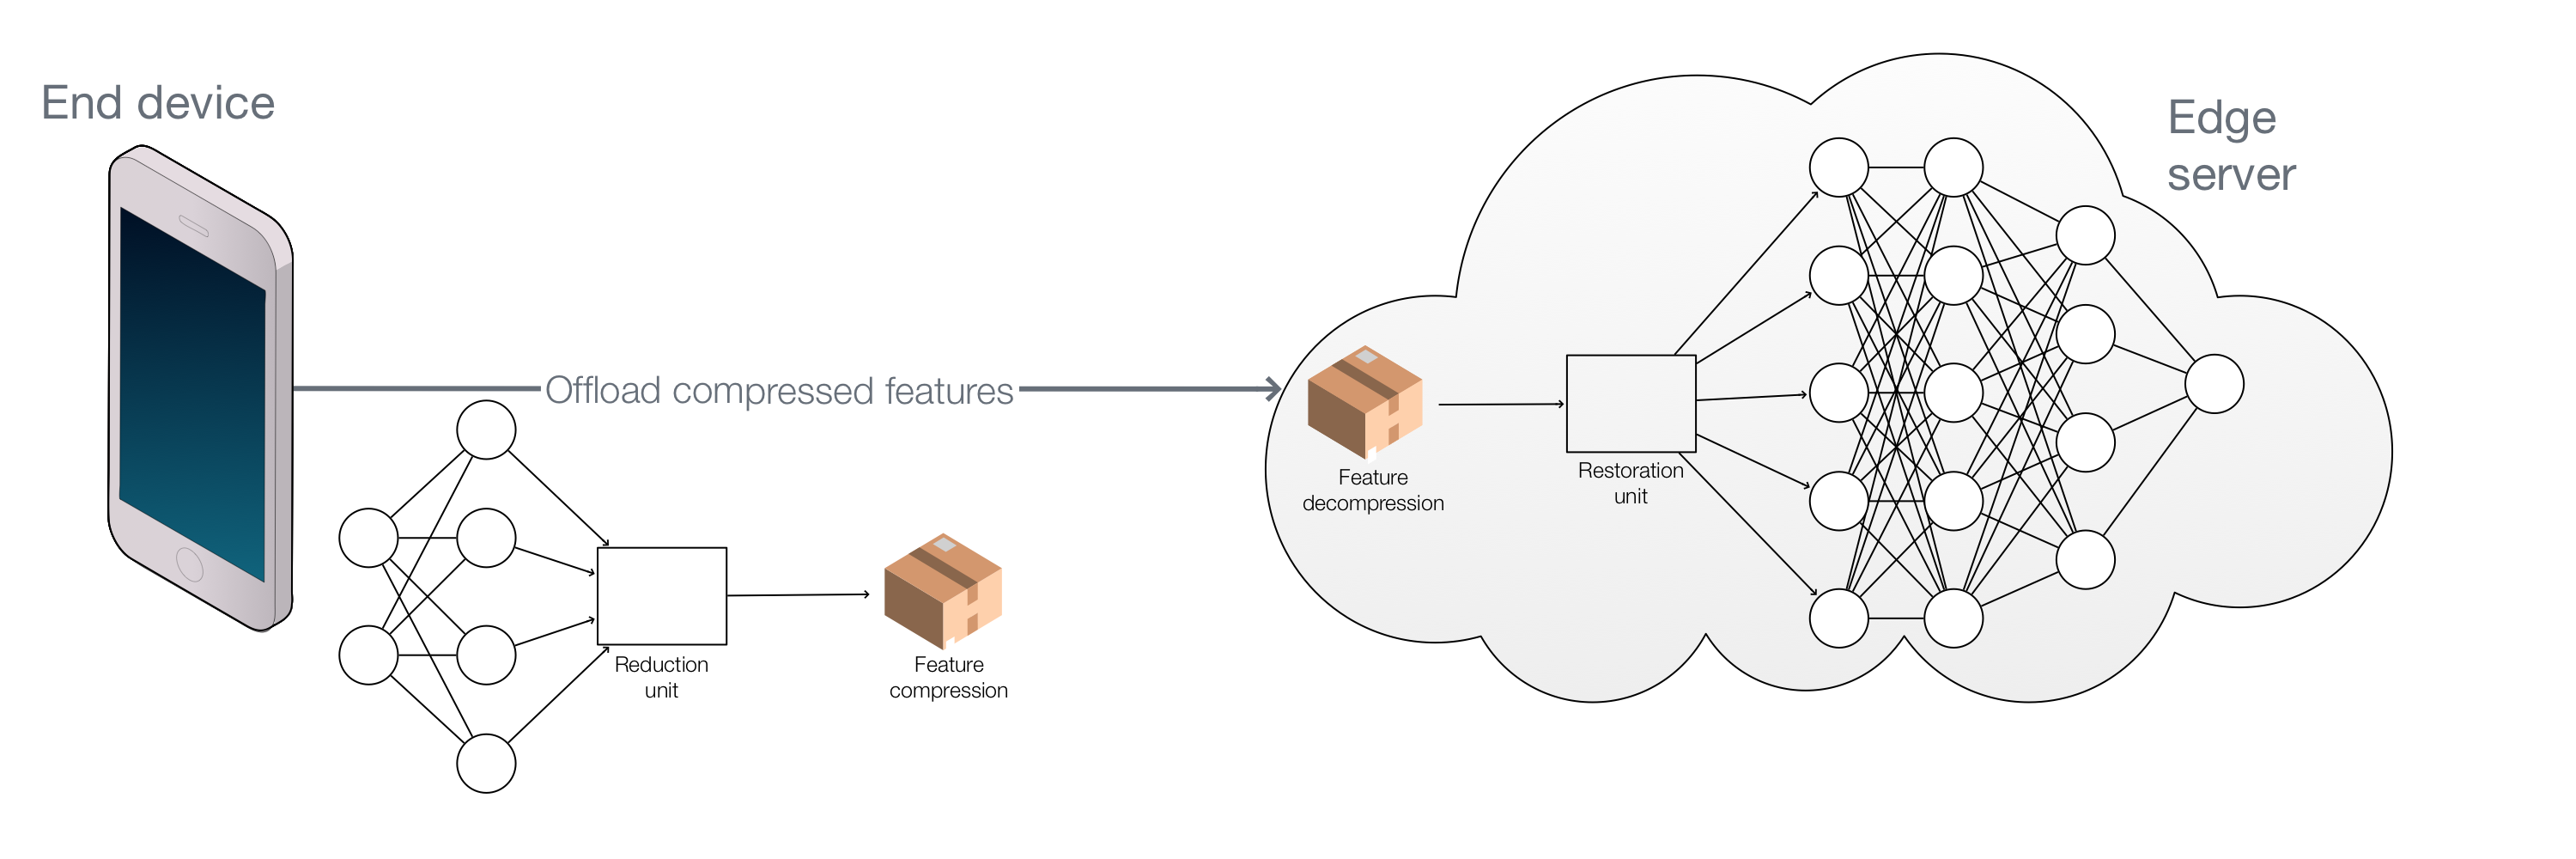
\includegraphics[width=\linewidth]{figures/models/bottlenet}
	\caption[BottleNet Unit]{BottleNet Unit}
\end{figure}

\gls{bottlenet} is able to achieve 84$\times$ bit savings compared to cloud-only approach with less than 2\% degradation of accuracy caused by lossy compression with compression-aware training. Under good networking condition, the evaluation of \gls{bottlenet} shows, that the best split is after the first convolutional block, as a smaller representation of the input can be found already here. Compared to cloud-only approach using WiFi a 8$\times$ speed up is found.

The collaborative scheme between end device and edge servers shows improvements for \gls{cpu}-enabled end devices, compared to a cloud-only approach, however as communication is introduced the overall latency will vary depending on the networking conditions. Model selection is an approach, that tries to limit the amount of offloading, by first running an on-device model. 

\subsection{Model Selection}

Model selection is an approach to reduce inference by selecting an appropriately accurate model, hence not using an unnecessarily deep model, if a shallower model should be satisfiable. In \cite{bolukbasi_adaptive_2017} a model selection framework is proposed. The framework stacks three increasingly deeper and more accurate models on top of each other; \gls{alexnet}, \gls{googlenet} and \gls{resnet}50. 

\begin{figure}
	\centering
	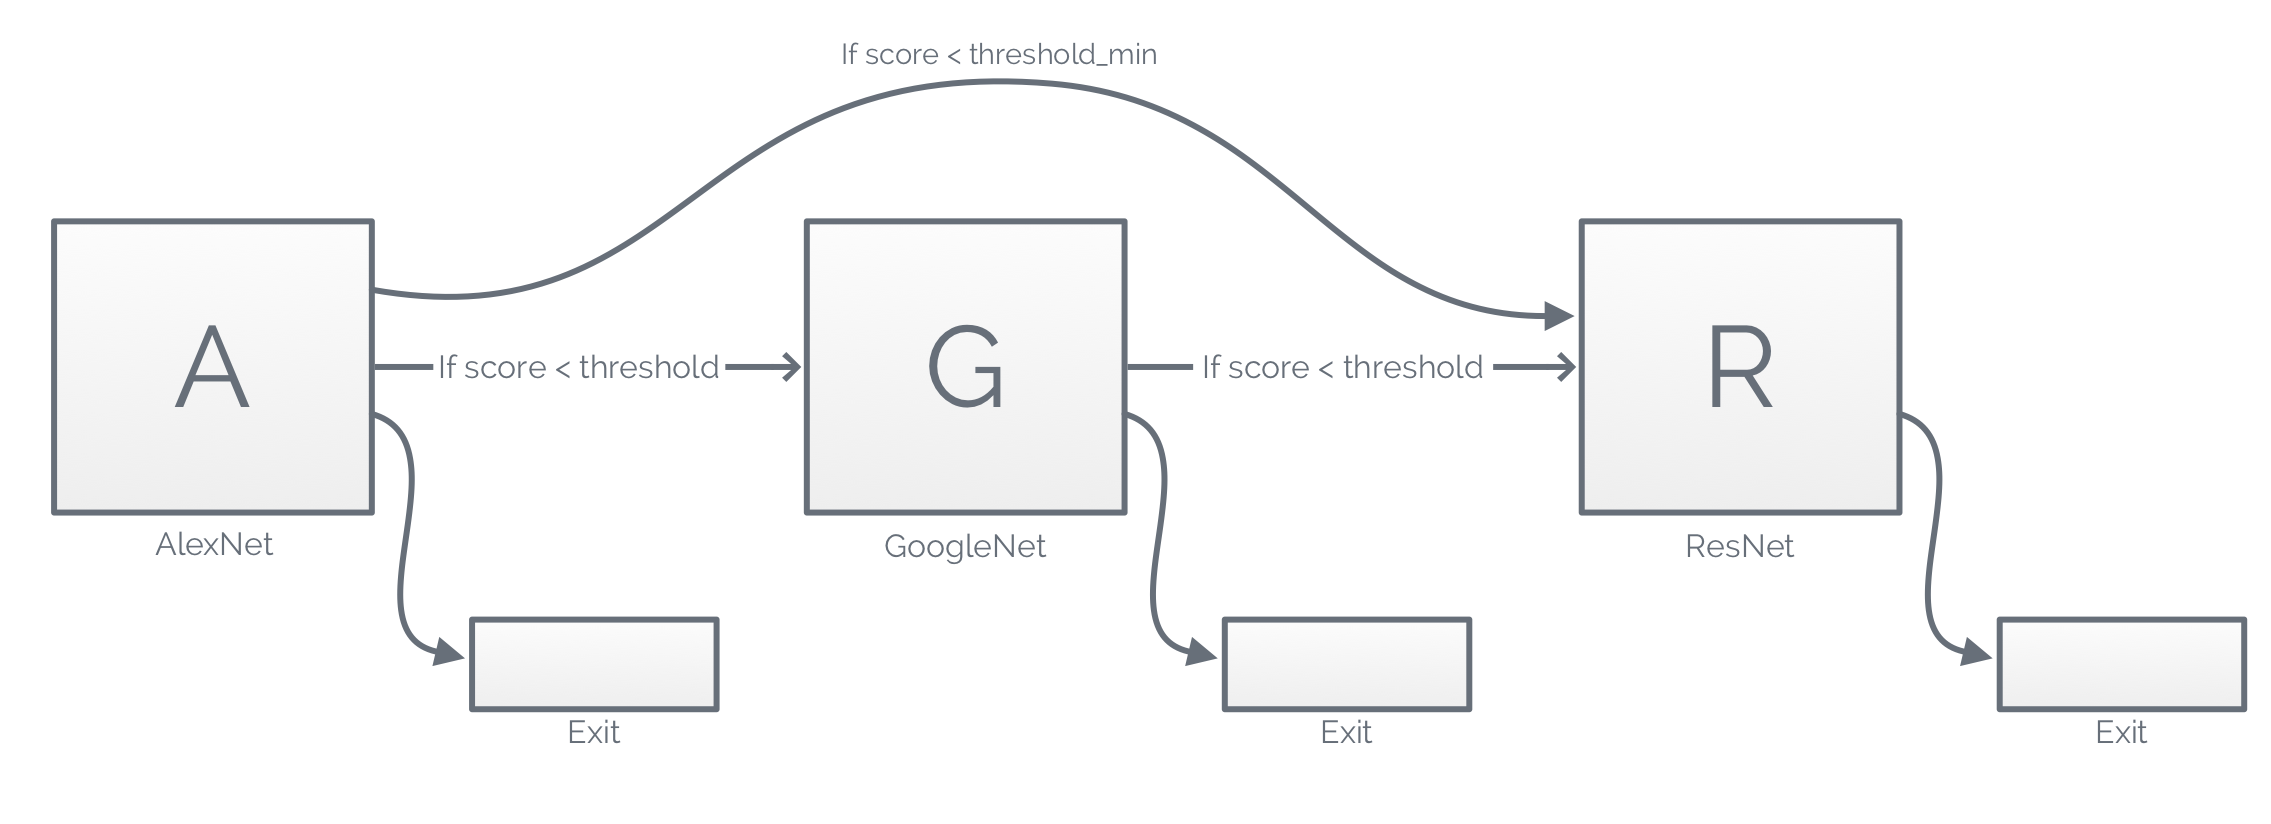
\includegraphics[width=\linewidth]{figures/models/adaptive}
	\caption[Adaptive Neural Network]{Adaptive Neural Network using model selection}
\end{figure}

The input is inferred to \gls{alexnet}, if the confidence scores is satisfactory the prediction is accepted, if not the framework decides to use either \gls{googlenet} or \gls{resnet}50 depending on a confidence threshold, however if the sample is inferred to \gls{googlenet} and the confidence is still unsatisfactory the sample is inferred to \gls{resnet}50 for the final prediction. The work shows improvement of the average prediction time with only a small reduction in accuracy depending on the confidence threshold. However, for hard samples, since multiple model are introduced, the inference time is increased, as well as the computational cost and memory consumption, thus such model selection approach seems overwhelming to introduce on an end-device yet it may be feasible in an edge-device mode using a Big/Little setup.

To obtain faster inference Big/Little \gls{dnn} \cite{park_big/little_2015} is simple approach using model selection. It implements a hybrid edge architecture of device-only and selective offloading for edge-only processing. It runs a smaller yet less accurate model on device and a larger more accurate model on the edge server, as illustrated by figure \ref{fig:big/little-dnn}. 

\begin{figure}
	\centering
	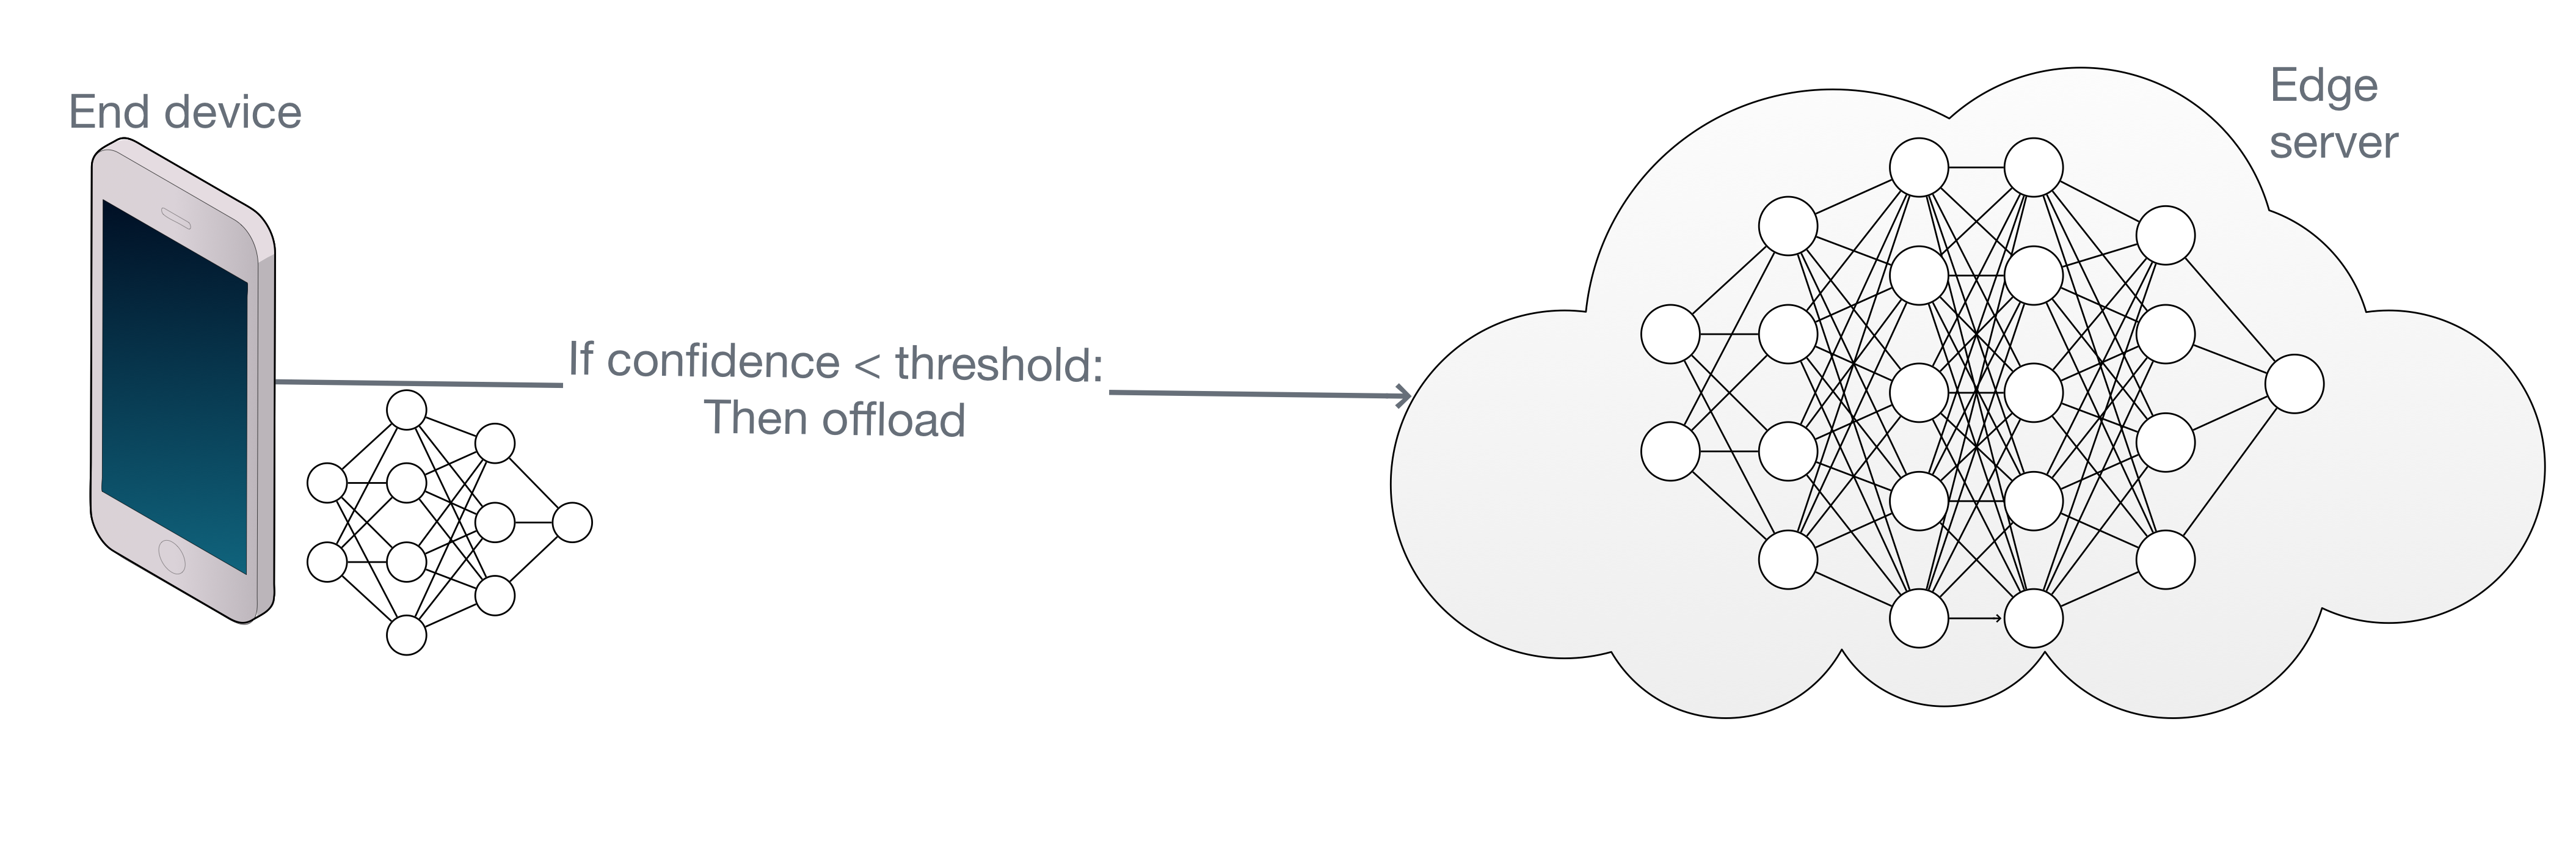
\includegraphics[width=\linewidth]{figures/models/big_little_dnn}
	\caption[Big/Little \gls{dnn} architecture]{Big/Little \gls{dnn}, a hybrid edge architecture. An on-device model is used to selectively offload to a more complex model hosted on an edge server.}
	\label{fig:big/little-dnn}
\end{figure}

If the prediction confidence of the little model is unsatisfactory, a decision is made to offload to the big model on the edge server. If a lot of samples are able to be correctly classified locally a speed-up is gained. However, the down-side of this approach is, if too many samples require the big model to satisfy a certain confidence threshold, a lot of work is wasted on the on-device prediction. Nonetheless the paper \cite{park_big/little_2015} contribute with another method to define a threshold, called \textsc{Score margin}. They have found, that the difference between the highest scoring and second highest scoring prediction, have a close relation to the actual true label. Although Big/Little \gls{dnn} obtain good results on energy savings and inference latency, more sophisticated frameworks such as early exiting, that also enabled model partitioning have been proposed.

\subsection{Model Early Exit}

Model early exiting is a way to handle the latency-accuracy trade-off, by reducing the average inference time without compromising model accuracy. Typically samples can be accurately classified using less \gls{dnn} layers which can improve the inference time, if a sample cannot be classified with proper confidence more layers can be used to obtain a more confident prediction. Since early exiting less computation is wasted, if offloading is necessary after an exit compared to a Big/Little model selection setup. As less computation is needed and a smaller representation of input data can be obtained, thus less data must be offloaded to the edge server.

Cascading neural networks \cite{leroux_resource-constrained_2015} by \citeauthor{leroux_resource-constrained_2015} proposes an early exiting framework by adding a cascade of intermediate classifiers, that allow some sample to exit the model early, hence improving inference time. \gls{branchynet} \cite{teerapittayanon_branchynet:_2016} proposed by \citeauthor{teerapittayanon_branchynet:_2016} is an early exiting framework for existing state-of-the-art model, that allow for fast inference. The paper proposes a novel joint optimization of the all output branches which shows added regularization to the model weights. The framework shows promising results of reduced inference time. The result are based on three well-known \gls{dnn} architectures; \gls{lenet} \cite{lecun_lecun-98.pdf_1998}, \gls{alexnet} \cite{krizhevsky_imagenet_2017} and \gls{resnet} \cite{he_deep_2015}, modified to implement the \gls{branchynet} framework, and to accommodate the MNIST \cite{lecun_mnist_2010} and Cifar-10 \cite{krizhevsky_cifar-10_nodate} datasets.

\begin{figure}
	\centering
	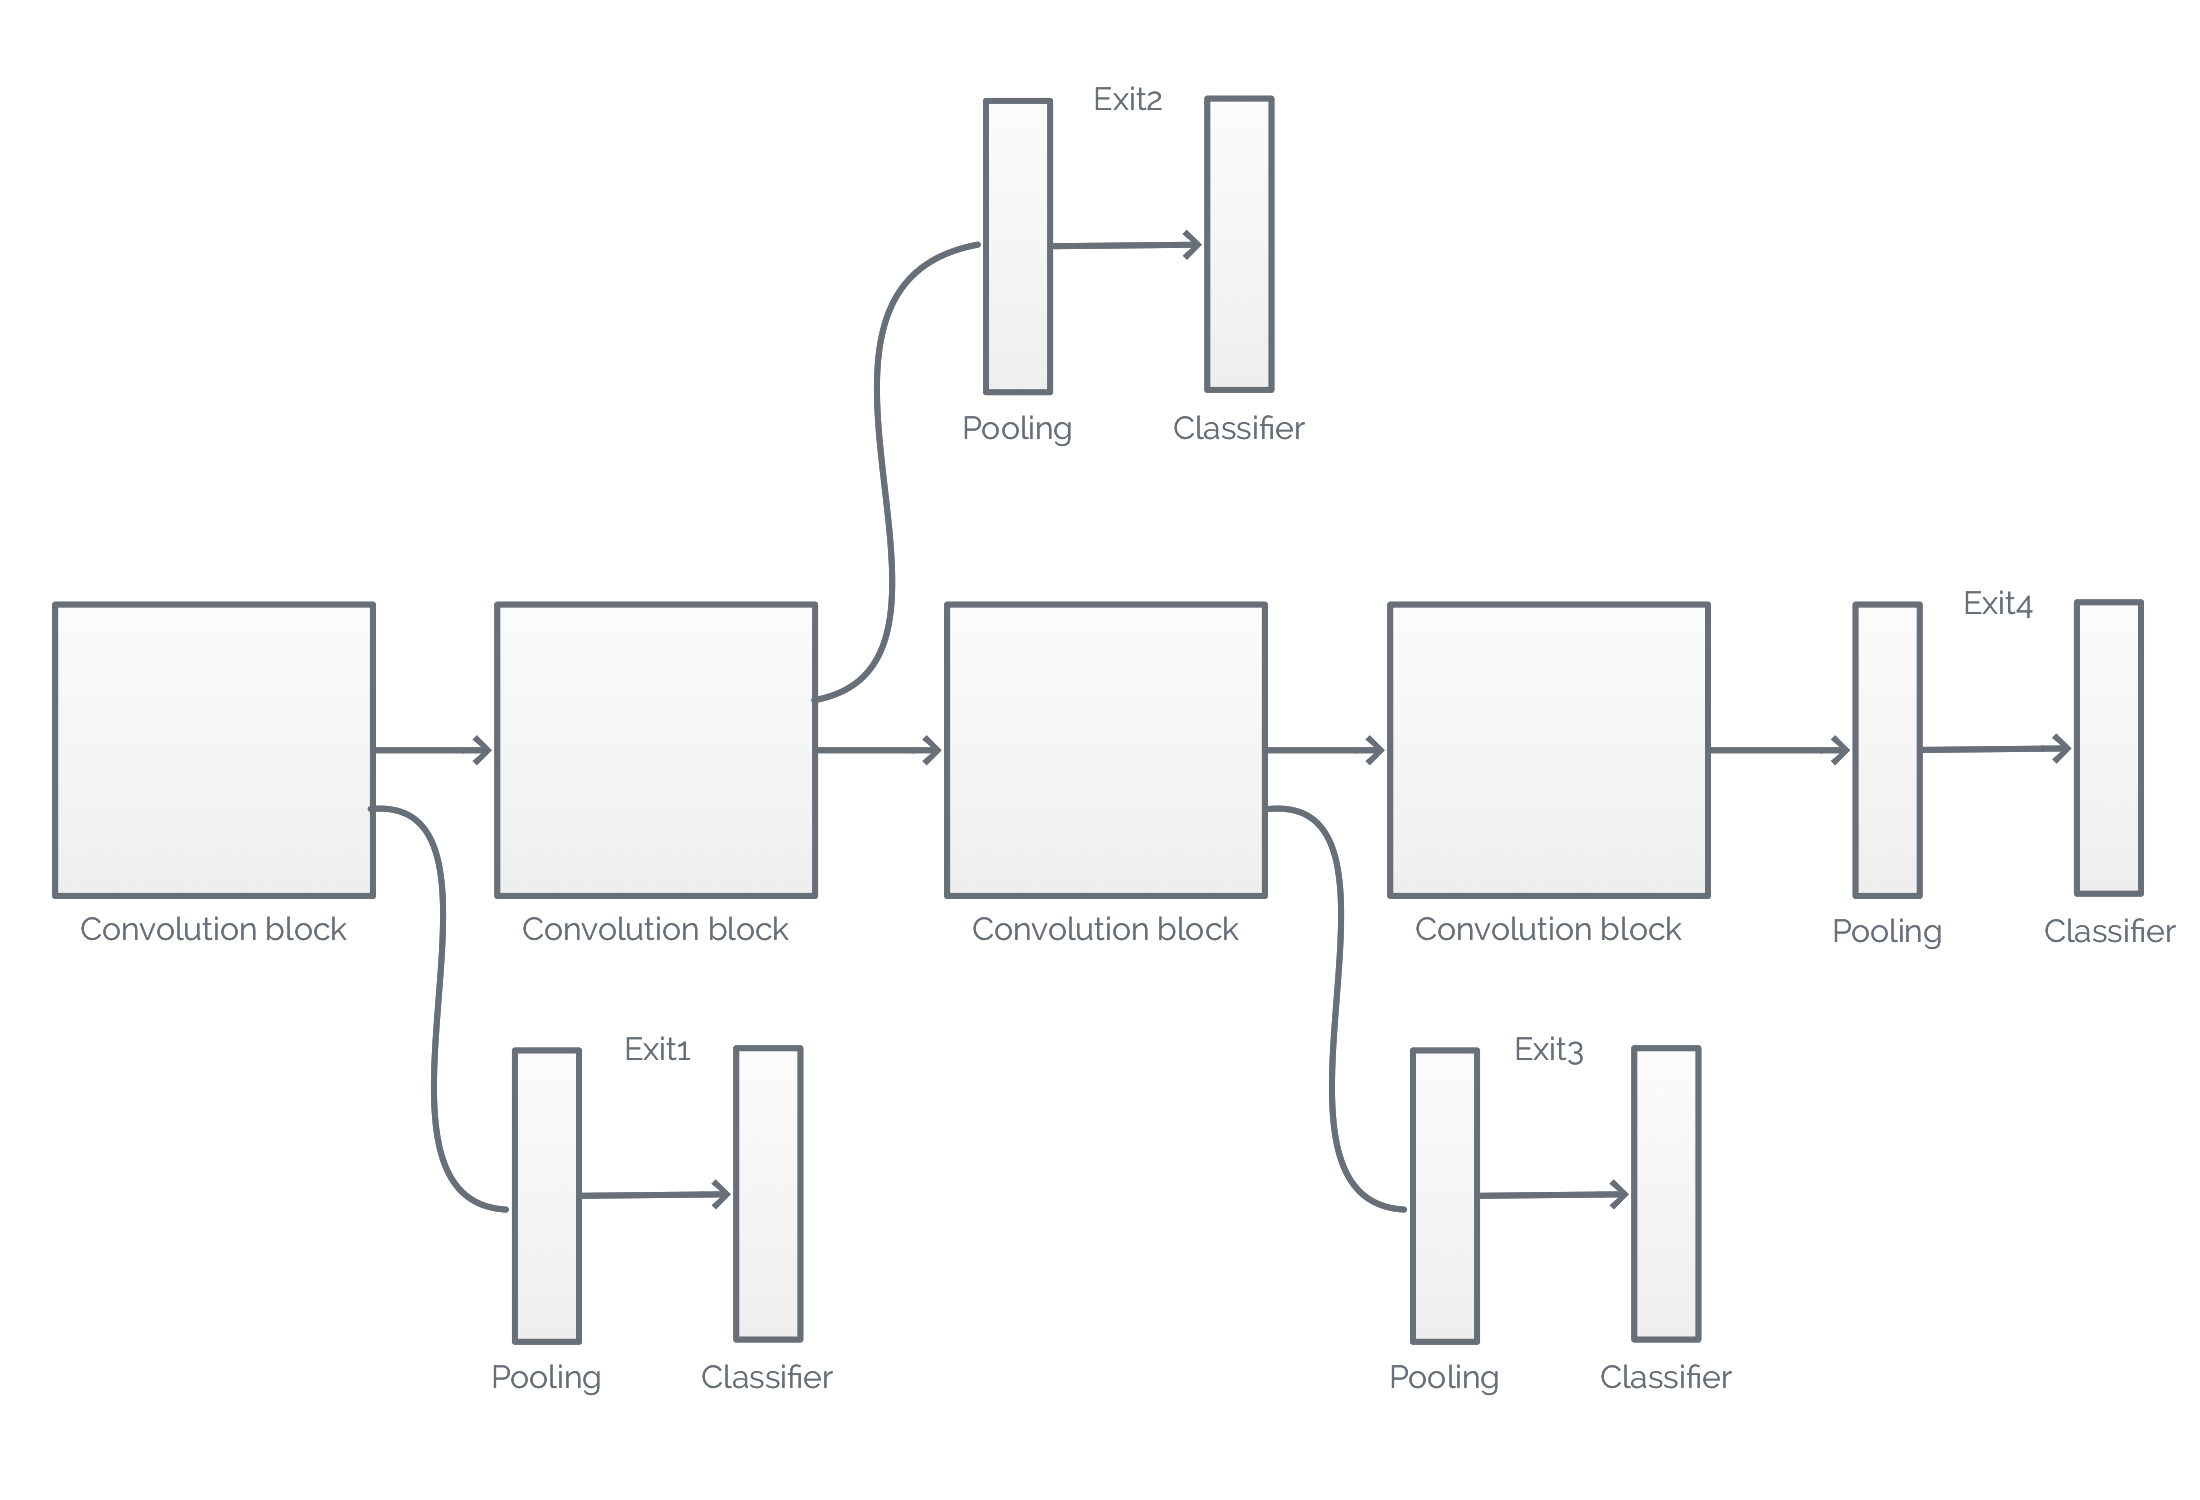
\includegraphics[width=\linewidth]{figures/models/branchy}
	\caption[BranchyNet Architecture]{BranchyNet Architecture}
\end{figure}

Cascading neural network \cite{leroux_resource-constrained_2015} have been followed up in \cite{leroux_cascading_2017} and \gls{branchynet} have been extended to \gls{ddnn} in \cite{teerapittayanon_distributed_2017}. Both papers are distributing the early exiting model over a distributed computing hierarchy over cloud, edge and end devices.  

The distributed cascading neural network and \gls{ddnn} is basically alike, however the papers have different perspectives. \gls{ddnn} focuses on a cluster of $k$ stationary end devices collaboratively solving a classification challenge using sensor fusion. In \gls{ddnn}  early exits are placed to create a shallow on device model. If of local recognition with satisfying confidence cannot be obtained, then the intermediate features of the early exit are offloaded to servers. The paper investigate different aggregation schemes and find a concatenation of features to be the best performing. Concatenation of features increases the size needed to be offloaded to servers, to $k$ times the amount of features at the exit point of the model. The \gls{ddnn} framework require complete retraining of the model, as the amount of features after the exit point is not consistent with the existing \gls{dnn} architecture or it will require new novel architectures optimized for the \gls{ddnn} framework. Nonetheless, the work shows benefits from distributed computing to provide fault tolerance and support for sensor fusion of geographically dispersed sensors to improve recognition accuracy.

Cascading neural network \cite{leroux_cascading_2017} on the other hand is more focused on reducing inference time of a single \gls{dnn} with early exiting, which is more suitable for mobile \gls{p2p} applications, however still cascaded/distributed over a computing hierarchy. Training the cascaded neural network is no different than training any other early exiting model, however in \cite{leroux_cascading_2017}, they freeze the network weights and only train the softmax classifiers, whereas in \cite{teerapittayanon_branchynet:_2016} show, that training the model's weights benefit from the joint optimization in the form of added regularization and obtaining early features more suited for early exiting. In the cascading neural network \cite{leroux_cascading_2017}, early exiting and network partitioning point can be chosen depending available networking bandwidth, yet the exit and partition point is assigned statically and evaluated at two different settings, where the point is placed at two different depths. 

\begin{figure}
	\centering
	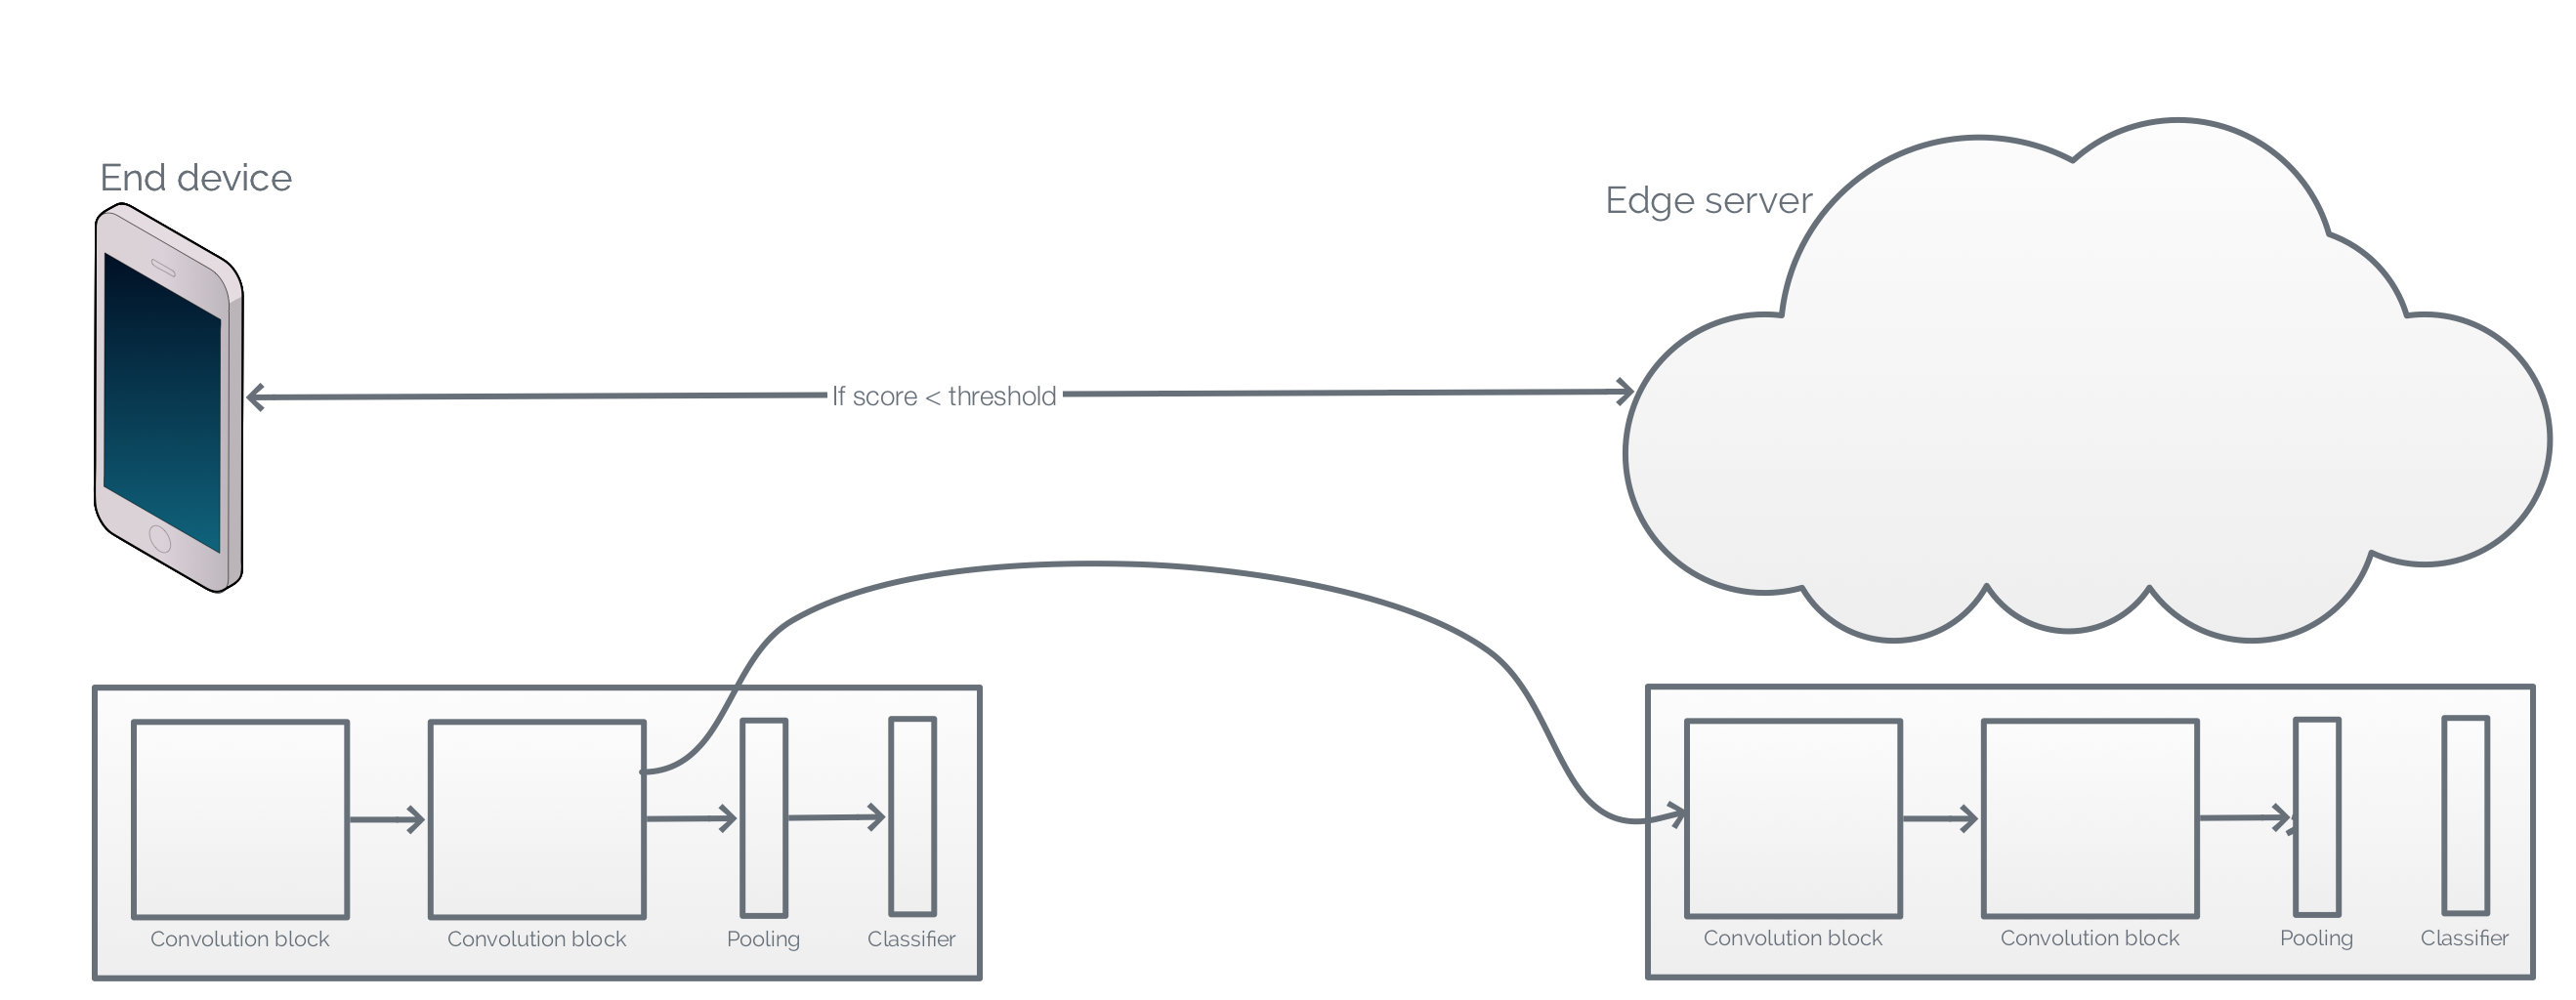
\includegraphics[width=\linewidth]{figures/models/cascaded}
	\caption[Cascaded \gls{dnn} over a computing hierarchy]{Cascaded \gls{dnn} over a computing hierarchy}
\end{figure}

Another proposal Edgent \cite{li_edge_2018} by \citeauthor{li_edge_2018} is a framework built on top of a \gls{branchynet} model. Edgent is an optimization of the latency-accuracy trade-off for mission-critical application with a predefined deadline. It tries to optimize the selection of exit and partitioning point of a cascaded early exiting model in the online phase. The optimization is based on a latency requirement, a regression model of each layer type of the used \gls{branchynet} model and the observed available bandwidth between end device and edge server. Experiments in the paper show, that Edgent is able to meet more stringent deadlines, than running solely on device or edge and naively selecting partitioning points. However, one may question whether Edgent is actually an early exiting framework, as the \gls{dnn} optimizer decides an exit and partitioning point upfront to use as much of available time budget as possible without violating the latency requirement, hence model selection. In a true early exiting some samples should be able to exit early, thus when \gls{dnn} is cascaded over the network, some samples should be able to exit locally on end devices to reduce expensive cost of network communication in terms of both latency and energy usage. When using a powerful edge server more weight will be added to offloading and no savings are gained on easy samples and the accuracy of harder samples are degraded. Edgent as a model selection framework is still a significant contribution for time-critical applications.

On a per model level \citeauthor{huang_multi-scale_2017} have in \cite{huang_multi-scale_2017} investigated different state-of-the-art architectures for early exiting. They have found, that  densely connected layers of \gls{densenet} \cite{huang_densely_2016} are more suitable for early exiting than the popular \gls{resnet} architecture build of residual blocks. Densely connected block uses a concatenation of features from all layers for final classification. The combination of  general feature and increasingly more specific and complex features are shown to be important for early exiting models. This finding have been used to come of with a novel \gls{dnn} archtiecture specifically designed for early exiting. \gls{msdnet} \cite{huang_multi-scale_2017} uses the densely connected layers along with multi-scale paths. The unique design of multi-scale densely connected blocks shows further improvement on early exiting.

\begin{figure}
	\centering
	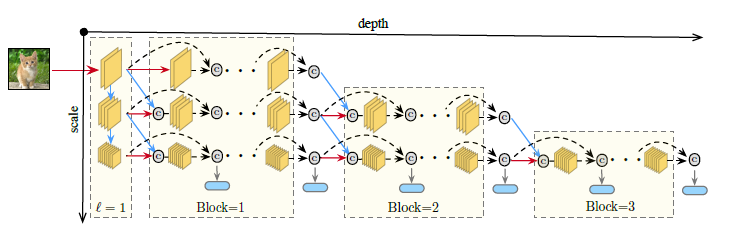
\includegraphics[width=\linewidth]{figures/models/msdnet}
	\caption[\gls{msdnet} Architecture]{\gls{msdnet} Architecture, Source: \citetitle{huang_multi-scale_2017} \cite{huang_multi-scale_2017}}
\end{figure}

\subsection{Model Layer Skipping}

Other approaches to reduce inference time of \gls{dnn} involve mechanism for skipping certain layers. SkipNet \cite{wang_skipnet:_2017} is a framework for adding dynamic decision for skipping layers. 

\begin{figure}
	\centering
	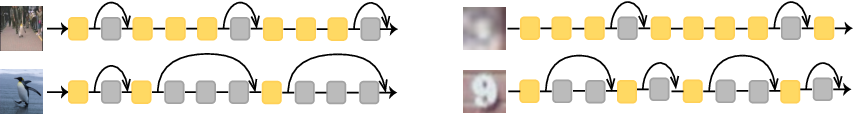
\includegraphics[width=\linewidth]{figures/models/skipnet}
	\caption[SkipNet]{SkipNet}
\end{figure}

The framework adds complexity to the model by introducing skipping gates between intermediate layers of the network. SkipNet is trained using a hybrid of supervised learning and reinforcement learning. The classification is learnt as a usual supervised problem using labeled data. The skipping policies are learnt using reinforcement learning by rewarding decision, that have little impact on classification accuracy. The work shows, that only a small fraction of inputs actually require extremely deep models, thus being able to reduce computational cost by 30\% of \gls{resnet}101 on \gls{ilsvrc2012}. 

BlockDrop \cite{wu_blockdrop:_2017} is another approach to learn skipping policies. However, instead of adding intermediate skipping gates for dynamic local decisions, BlockDrop trains a global policy network, that selectively chooses which model depth to use. BlockDrop is in fact a model selection framework, where the selection of models are learnt rather than tested. 

\begin{figure}
	\centering
	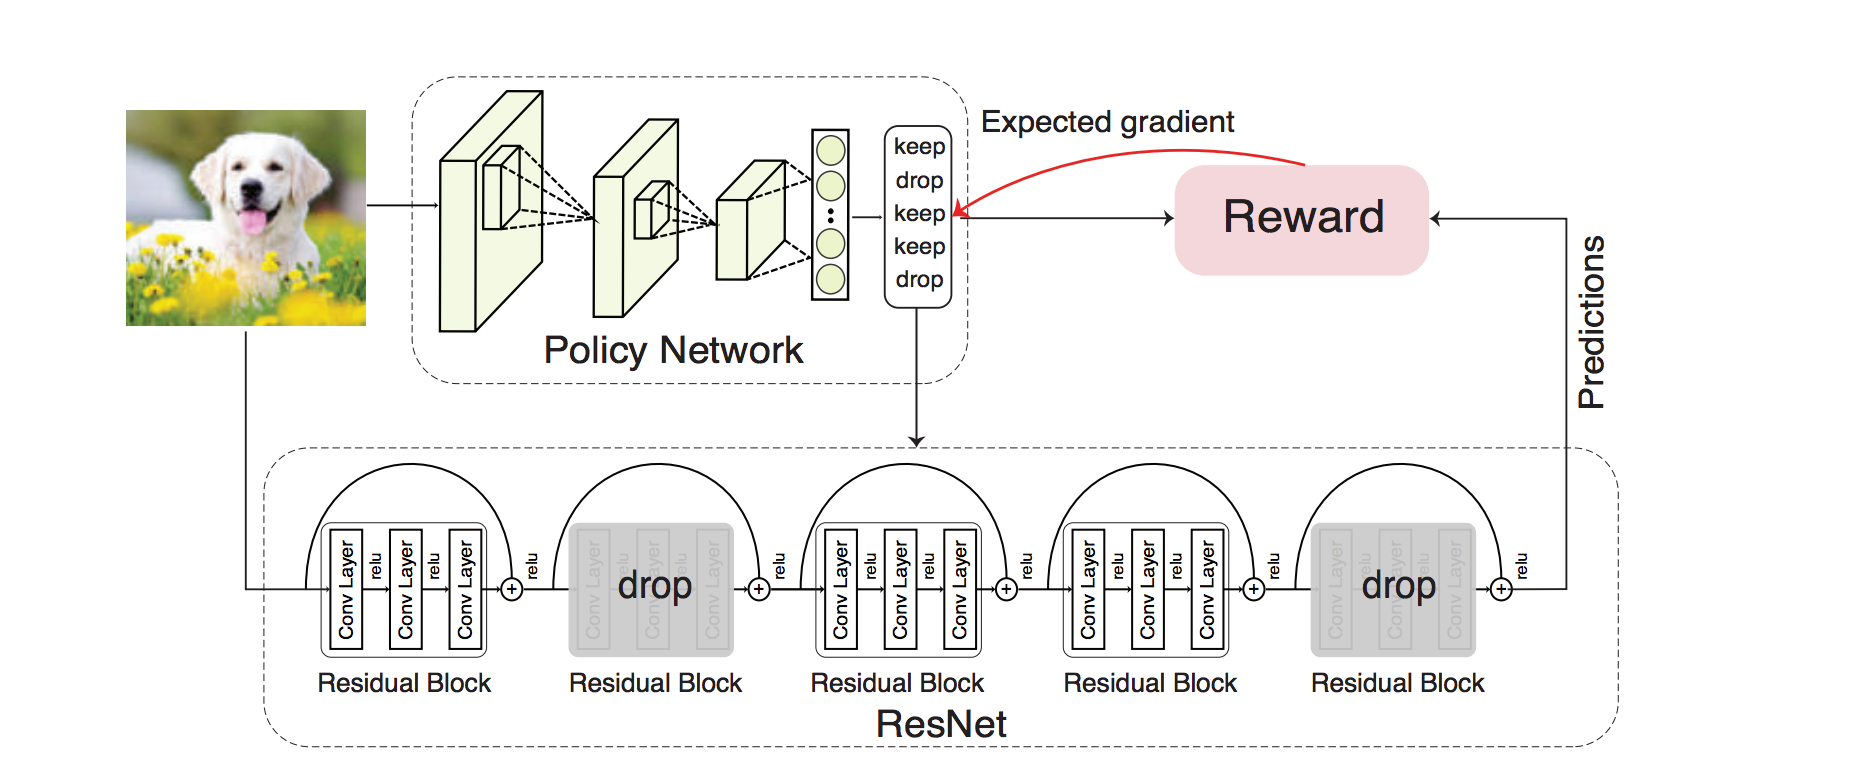
\includegraphics[width=\linewidth]{figures/models/blockdrop}
	\caption[BlockDrop]{BlockDrop}
\end{figure}

The policy network is similarly trained using reinforcement learning. The training shows, which classes are easy and which are hard. SkipNet and BlockDrop could both be used in an edge-device mode although neither architecture support early exiting or cascading, but would be useful in a Big/Little \cite{park_big/little_2015} setup. Particularly BlockDrop where the policy network run by an end device would selective choose among a smaller model on device or a larger model on an edge server to avoid wasteful execution of a smaller model.

\section{Our contribution}

We look at combining early exiting with model partitioning. 

The objective of this thesis is, taking mobile AR applications as use case, to design and implement of MEC offloading deep learning algorithms to maximize the inference reliability while meeting the service latency deadline. The thesis will design feasible offloading schemes, such as deep neural network partitioning, preprosssing (feature extractions), in objective detection and classification. The proposed schemes will be implemented using Raspberry Pi and Jetson TX2. The communication and computation latency, as well as the inference accuracy and reliability will be measured and analyzed.